\documentclass[a4j,11pt,titlepage]{jarticle}
\usepackage[%
	paper=a4paper,%
	textwidth=440pt,%
	textheight=715.5pt,%
	centering,%
	headheight=2zh,%
	footskip=2zh]{geometry}

\usepackage{amsmath,amssymb,amsopn,amsthm}
\usepackage{thmtools}
\usepackage{comment}
\usepackage[shortlabels]{enumitem}
\usepackage[dvipdfmx]{xcolor}
\usepackage{cite}
\usepackage[dvipdfmx]{graphicx}
\usepackage[hang]{subfigure}
\usepackage[subfigure]{ccaption}
\usepackage[nottoc,section]{tocbibind}
\usepackage{url}
\usepackage{listings,jlisting}
\usepackage{mathtools}

% 文書のプロパティ
\title{Pythonプログラミングの手引き}
\author{%
\begin{tabular}{rl}
京都大学大学院情報学研究科
&	今井貴史\\
&	後藤貴宏\\
&	石田達大\\
&	小山和輝\\[1ex]
京都大学工学部情報学科
&	枡井啓貴
\end{tabular}}
\date{\today}

% フォント
%\usepackage[expert]{otf}
%\usepackage{pxfonts}
%\usepackage{txfonts}
%\delimiterfactor=901
%\delimitershortfall=5pt
\usepackage{fourier-orns}
\usepackage{fontawesome}
\usepackage{yhmath}

% 演算子
\DeclareMathOperator\diff{d\!}
\DeclareMathOperator\ddiff{d^2\!}
\makeatletter
\DeclareMathOperator{\@diff}{d}
\newcommand{\ndiff}[1]{\@diff^{#1}\!}
\makeatother
\DeclareMathOperator\Diff{D\!}
\DeclareMathOperator\grad{grad}
\DeclareMathOperator\Real{Re}
\DeclareMathOperator\Imag{Im}
\DeclareMathOperator\atantwo{atan2}
% 数学定数
\def\I{\mathord{I}}
\def\i{\mathord{\mathrm{i}}}
\def\e{\mathord{\mathrm{e}}}
\def\cpi{\mathord{\mathrm{\pi}}}
%\def\cpi{\mathord{\pi}}
% その他
\def\set#1{\mathbb{#1}}
\def\point#1{\mathrm#1}
\def\Vec#1{\boldsymbol{#1}}
%\def\T#1{\mathord{\mathopen{{\vphantom{#1}}^\mathrm{t}}#1}}
\def\T#1{{#1}^\top}
\def\norm#1{\left\lVert #1 \right\rVert}
\def\wildcard{\mathord{\,\cdot\,}}
\def\ol#1{\overline{#1}}

% 定理環境
\newtheoremstyle{lite}%
	{5pt}%	Space above
	{5pt}%	Space below
	{}%	Body font
	{}%	Indent amount
	{\normalfont}%	Theorem head font
	{}%	Punctuation after theorem head
	{.5em}%	Space after theorem head
	{\thmname{#1}\thmnumber{ #2}\thmnote{ (#3)}}%	Theorem head spec

\theoremstyle{lite}
\definecolor{attentionbgcolor}{gray}{.9}
\declaretheorem[%
	name={{\Large \danger}},%
	numbered=no,%
	shaded={%
		bgcolor=attentionbgcolor,%
		margin=10pt}]%
	{attention}

% 表紙スタイル
\definecolor{titlecolor}{cmyk}{1,.60,0,.40}
\makeatletter
\renewcommand{\maketitle}{\begin{titlepage}%
	\newgeometry{textwidth=440pt,textheight=600pt,centering}
	\raggedright
	{\Huge\bfseries \textcolor{titlecolor}{\@title} \par}
	\vspace{2cm}
	\raggedleft
	{\Large \@author \par}
	\vfill
	\centering
	{\large \@date \par}
	\end{titlepage}%
	\restoregeometry}
\makeatother

% 見出しスタイル
\usepackage{titlesec}
\titlelabel{\S\;\thetitle.\quad}
\setcounter{secnumdepth}{3}
\titleformat{\subsubsection}{}{\thesubsubsection}{.5em}{}
\renewcommand{\thesubsubsection}{\alph{subsubsection})}
\setcounter{tocdepth}{2}

% 脚注スタイル
\makeatletter
\def\thefootnote{\ifnum\c@footnote>\z@\leavevmode\lower.5ex%
  \hbox{$^{\dagger\@arabic\c@footnote}$}\fi}
\makeatother

% 参考文献スタイル
\tocotherhead{subsection}

% ソースコードスタイル
\renewcommand{\lstlistingname}{コード}
\lstdefinestyle{cmdline}{%
	language=bash,
	basicstyle=\ttfamily\small,%
	commentstyle=\color[rgb]{0,0.5,0},%
	frame=single,%
	showstringspaces=false,%
	numbers=none}
\lstdefinestyle{python}{%
	language=python,
	basicstyle=\ttfamily\small,%
	commentstyle=\color[rgb]{0,0.5,0},%
	frame=single,%
	showstringspaces=false,%
	numbers=left}

% キャプションスタイル
\hangcaption

% 数式番号スタイル
\numberwithin{equation}{section}

% 数式スタイル
\allowdisplaybreaks[4]

% ページスタイル
\usepackage{fancyhdr}
\pagestyle{fancy}
\renewcommand{\sectionmark}[1]{%
	\markboth{\S\;\thesection.{\quad}#1}{}}
\fancypagestyle{cover}{%
	\lhead{}
	\chead{}
	\rhead{}
	\lfoot{}
	\cfoot{}
	\rfoot{}
	\renewcommand{\headrulewidth}{0pt}
	\renewcommand{\footrulewidth}{0pt}
}
\fancypagestyle{toc}{%
	\lhead{}
	\chead{}
	\rhead{}
	\lfoot{}
	\cfoot{}
	\rfoot{}
	\renewcommand{\headrulewidth}{0pt}
	\renewcommand{\footrulewidth}{0pt}
}
\fancypagestyle{body}{%
	\lhead{\nouppercase\leftmark}
	\chead{}
	\rhead{\nouppercase\rightmark}
	\lfoot{}
	\cfoot{\thepage}
	\rfoot{}
	\renewcommand{\headrulewidth}{.4pt}
	\renewcommand{\footrulewidth}{0pt}
}

%%%%%%    TEXT START    %%%%%%
\begin{document}
\onecolumn
\thispagestyle{cover}
% 表紙
\maketitle
%\input{title}

\clearpage
\onecolumn
\pagenumbering{roman}
\pagestyle{toc}
% 目次
\tableofcontents

\clearpage
\onecolumn
\pagenumbering{arabic}
\pagestyle{body}
% 本文はここから


% Python環境の構築手順
\section{Python環境の構築手順}\label{sec: Python環境の構築手順}
本節ではデータ解析プラットフォームAnacondaの導入手順を説明する.
AnacondaはPythonのディストリビューションの一つであり,
その最大の特徴はデータ解析に有用な追加パッケージを多数そろえていることにある.
また,それらのパッケージの間の依存関係を処理するために
独自のパッケージ管理システムCondaが用意されていることも特徴の一つである.
Condaを用いることで,パッケージの導入・アップデート・削除のほか,
Python仮想環境の構築・管理なども容易に行うことが可能となる\footnote{%
この辺りの詳細については
公式ドキュメント
(\url{http://conda.pydata.org/docs/index.html})
などを参照されたい.
}.


\subsection{Windowsの場合}


\subsubsection{新規インストール}
\begin{enumerate}
\item
公式サイトのダウンロードページ
(\url{https://www.continuum.io/downloads/})
から自分のWindows環境($32$ビット版/$64$ビット版)\footnote{%
コントロールパネルから[システム]を開き,「システムの種類」で確認可能.
}に合ったインストーラをダウンロードする.
\item
ダウンロードしたインストーラを実行し,
表示された指示に従ってインストールする.
\end{enumerate}

\begin{attention}
ほかのPythonディストリビューション(ActivePythonなど)が
インストールされている場合,
Anacondaをインストールしても,
設定によっては前者が優先的に使用されてしまう.
優先順位を確認するためには,
コマンドプロンプト(cmd.exe)上で次のコマンドを実行すればよい.
\begin{lstlisting}[style=cmdline]
> where python.exe
\end{lstlisting}
このコマンドの出力の先頭行にAnaconda以外のPythonが表示されたときは,
以下の手順で
AnacondaのPythonが優先的に使用されるように変更する.
\begin{enumerate}
\item
コントロールパネルから
[システム]→[システムの詳細設定]→[環境変数]と進み,
システム環境変数の「Path」を選択して[編集]ボタンを押す.
\item
変数値からAnaconda関係のエントリを切り取り,
ほかのPythonディストリビューションに関するエントリより前に貼り付ける.
\item
[OK]ボタンを押して設定を保存・反映させる.
\end{enumerate}
\end{attention}

\begin{attention}
Cygwin Terminal上では
Windowsの「Path」の前に\verb|/usr/local/bin:/usr/bin|が自動で追加され,
CygwinのPythonが優先的に使用されてしまう.
Cygwin Terminal上でも
デフォルトでAnacondaのPythonが使用されるようにするためには,
Cygwin Terminal上でさらに次のコマンドを実行する.
\begin{lstlisting}[style=cmdline]
$ echo 'export PATH=<Anaconda directory>:$PATH' >> ~/.bashrc
$ echo "alias python='python -i'" >> ~/.bashrc
\end{lstlisting}
%Cygwin TerminalからAnacondaのPythonを呼び出す際には,
%\verb|cygstart|コマンドを使用して次のようにすべきであろう.
%\begin{lstlisting}[style=cmdline]
%$ cygstart <Anaconda directory>/python
%\end{lstlisting}
ここで,\verb|<Anaconda directory>|には
AnacondaのインストールディレクトリをCygwin形式で記入すること
(例えば\verb|/cygdrive/c/Anaconda3|).
Cygwin Terminalを開きなおせば,
AnacondaのPythonが優先されるようになっているはずである.
\end{attention}


\subsubsection{旧バージョンからのアップデート}
コマンドプロンプト(cmd.exe)を開き,以下の手続きを実行する.
\begin{enumerate}
\item
パッケージ管理システム自体をアップデートする.
\begin{lstlisting}[style=cmdline]
> conda update conda
\end{lstlisting}
\item
パッケージ群をアップデートする.
\begin{lstlisting}[style=cmdline]
> conda update anaconda
\end{lstlisting}
\end{enumerate}


\subsection{Mac OS Xの場合}
\begin{attention}
Mac OS Xに関しては,
公式インストーラを用いてAnacondaを導入したところ
Condaがほかのパッケージ管理システムと衝突した,
という事例が報告されている.
そこで,よりクリーンな導入方法として,
ここでは
パッケージ管理システムHomebrewとPythonバージョン管理ツールpyenvとを用いた
方法を紹介する.
\end{attention}


\subsubsection{新規インストール}
ターミナル(Bash\footnote{%
ターミナルとしてBash以外を使用している場合は
コマンドを適当に変更すること.
})を開き,以下の手続きを実行する.
\begin{enumerate}
\item
(OSをEl Capitanより前のバージョンからEl Capitan以降にアップデートした場合)
\verb|/usr/local|のパーミッションが書き換えられてしまっている可能性がある.
以下のコマンドでパーミッションを復元する.
\begin{lstlisting}[style=cmdline]
$ sudo chown -R $(whoami):admin /usr/local
\end{lstlisting}
\item
(プロキシを介してインターネットを利用している場合)
環境変数でプロキシを指定する.
\begin{lstlisting}[style=cmdline]
$ export http_proxy=http://<proxyhost>:<proxyport>
$ export https_proxy=https://<proxyhost>:<proxyport>
\end{lstlisting}
ここで,\verb|<proxyhost>|にはプロキシのURL,
\verb|<proxyport>|にはプロキシのポート番号を記入すること.
\item
\begin{description}[font=\normalfont,style=sameline]
\item[(Homebrewがインストールされていない場合)]
\leavevmode
\begin{enumerate}[(i)]
\item
Command Line Tools for Xcodeをインストールする.
\begin{lstlisting}[style=cmdline]
$ xcode-select --install
\end{lstlisting}
\item
Homebrewをインストールする\footnote{%
Xcodeのライセンスに同意していないことで警告が出た場合,
表示された指示に従ってライセンスに同意する.
}.
\begin{comment}
\begin{lstlisting}[style=cmdline]
$ ruby -e "$(curl -fsSL \
	https://raw.githubusercontent.com\
		/Homebrew/install/master/install)"
\end{lstlisting}
\end{comment}
\begin{comment}
\begin{lstlisting}[%
	style=cmdline,%
	escapechar=|]
$ ruby -e "$(curl|\textvisiblespace|-fsSL|\textvisiblespace|\
> https://raw.githubusercontent.com\
> /Homebrew/install/master/install)"
\end{lstlisting}
\end{comment}
\begin{lstlisting}[style=cmdline]
$ ruby -e "$(curl -fsSL https://raw.githubusercontent.com\
  /Homebrew/install/master/install)"
\end{lstlisting}
\end{enumerate}
\item[(Homebrewがすでにインストールされている場合)]
\leavevmode\\
Homebrew自体とパッケージ一覧をアップデートしたうえで,
全パッケージをアップデートする.
\begin{lstlisting}[style=cmdline]
$ brew update
$ brew upgrade
\end{lstlisting}
\end{description}
\item
Homebrewを用いてpyenvをインストールする.
\begin{comment}
\begin{lstlisting}[style=cmdline]
$ brew install pyenv
$ echo 'export PYENV_ROOT=/usr/local/var/pyenv' \
	>> ~/.bash_profile
$ echo 'eval "$(pyenv init -)"' >> ~/.bash_profile
$ source ~/.bash_profile
\end{lstlisting}
\end{comment}
\begin{comment}
\begin{lstlisting}[style=cmdline]
$ brew install pyenv
$ echo 'export PYENV_ROOT=/usr/local/var/pyenv' \
> >> ~/.bash_profile
$ echo 'eval "$(pyenv init -)"' >> ~/.bash_profile
$ source ~/.bash_profile
\end{lstlisting}
\end{comment}
\begin{lstlisting}[style=cmdline]
$ brew install pyenv
$ echo 'export PYENV_ROOT=/usr/local/var/pyenv' \
  >> ~/.bash_profile
$ echo 'eval "$(pyenv init -)"' >> ~/.bash_profile
$ source ~/.bash_profile
\end{lstlisting}
\item\label{enum: Mac OS Xへの新規インストール - Anacondaのインストール}
\begin{enumerate}[(i)]
\item
pyenvで導入可能なAnacondaのバージョン一覧を確認する.
\begin{lstlisting}[style=cmdline]
$ pyenv install --list | grep 'anaconda3'
\end{lstlisting}
\item
pyenvを用いてAnacondaをインストールし,
さらにデフォルトのPython環境として設定する.
\begin{lstlisting}[style=cmdline]
$ pyenv install anaconda3-<Anaconda version>
$ pyenv global anaconda3-<Anaconda version>
$ pyenv rehash
\end{lstlisting}
ここで,\verb|<Anaconda version>|には
インストールしたいAnacondaのバージョンを記入すること.
特に理由がなければ
最新版(2016年7月21日の時点では\verb|4.0.0|)
を指定すればよい.
\end{enumerate}
\end{enumerate}


\subsubsection{旧バージョンからのアップデート}
ターミナル(Bash)を開き,以下の手続きを実行する.
\begin{enumerate}
\item
(OSをEl Capitanより前のバージョンからEl Capitan以降にアップデートした場合)
\verb|/usr/local|のパーミッションが書き換えられてしまっている可能性がある.
以下のコマンドでパーミッションを復元する.
\begin{lstlisting}[style=cmdline]
$ sudo chown -R $(whoami):admin /usr/local
\end{lstlisting}
\item
(プロキシを介してインターネットを利用している場合)
環境変数でプロキシを指定する.
\begin{lstlisting}[style=cmdline]
$ export http_proxy=http://<proxyhost>:<proxyport>
$ export https_proxy=https://<proxyhost>:<proxyport>
\end{lstlisting}
ここで,\verb|<proxyhost>|にはプロキシのURL,
\verb|<proxyport>|にはプロキシのポート番号を記入すること.
\item
Homebrew自体とパッケージ一覧をアップデートしたうえで,
全パッケージをアップデートする.
\begin{lstlisting}[style=cmdline]
$ brew update
$ brew upgrade
\end{lstlisting}
\item
pyenvを用いて
最新バージョンのAnacondaを新規インストールする.
(手順については新規インストールの
ステップ\ref{enum: Mac OS Xへの新規インストール - Anacondaのインストール}を
参照.)
\item
(必要に応じて)旧バージョンをアンインストールする.
\begin{enumerate}[(i)]
\item
インストールされているAnacondaのバージョン一覧を確認する.
\begin{lstlisting}[style=cmdline]
$ pyenv versions
\end{lstlisting}
\item
pyenvを用いてAnacondaをアンインストールする.
\begin{lstlisting}[style=cmdline]
$ pyenv uninstall anaconda3-<Anaconda version>
\end{lstlisting}
ここで,\verb|<Anaconda version>|には
アンインストールしたいAnacondaのバージョンを記入すること.
\end{enumerate}
\end{enumerate}


\subsection{動作テストのためのサンプルコード}
動作テストのために,
コード\ref{code: 動作テストのためのサンプルコード}にサンプルコードを掲載する.
実行すれば
(実行方法については第\ref{sec: Jupyter Notebookの使い方}節を参照)
図\ref{fig: サンプルコードの実行結果}のような結果が得られるはずである.

\lstinputlisting[%
	style=python,%
	label={code: 動作テストのためのサンプルコード},%
	caption={動作テストのためのサンプルコード.矩形波に対する三角多項式近似をプロットする.}]{code/sample.py}

\begin{figure}[htbp]
\centering
\setlength{\fboxsep}{0pt}
\fcolorbox{gray}{gray}{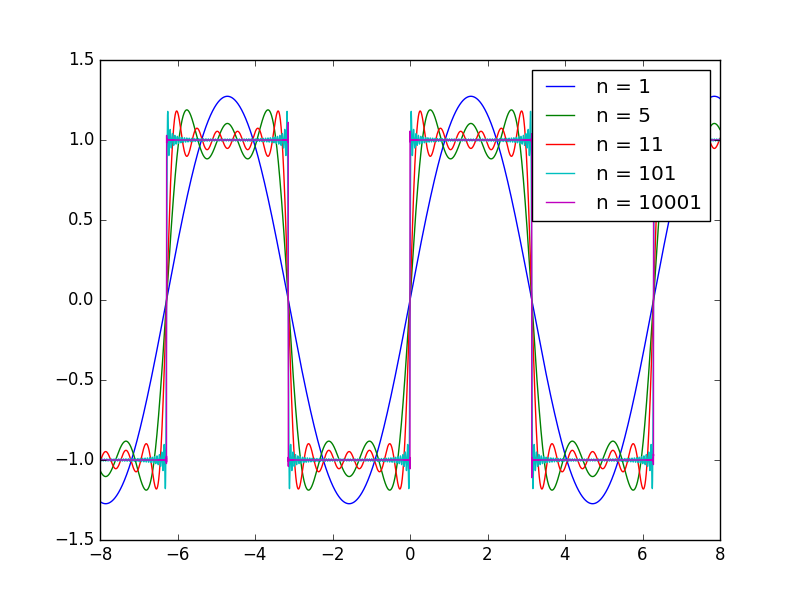
\includegraphics[scale=.4]{graphics/sample.png}}
\caption{\label{fig: サンプルコードの実行結果}%
コード\ref{code: 動作テストのためのサンプルコード}の実行結果.
}
\end{figure}


% Jupyter Notebookの使い方
\section{Jupyter Notebookの使い方}\label{sec: Jupyter Notebookの使い方}
Pythonを用いてデータ解析を行ううえでは,
対話的コンピューティング向けにPython標準のシェルを機能強化した
IPythonが有用である.
IPythonには
外部プログラムからIPythonの機能を利用するための機構が用意されている.
その機構を用いたIPythonのフロントエンドの一つがJupyter Notebookである.
本節ではJupyter Notebookを用いてPythonコードを編集・実行する方法を説明する.

なお,IPythonの機能を利用してPythonのコードを編集・実行するというのは
Jupyter Notebookにとって副次的な機能に過ぎない.
Jupyter Notebookの主たる機能は,
ノートブックとよばれる,
コードと出力を文章中に埋め込んだ文書を作成する機能である.
この機能の詳細については
参考文献\cite{rossant2015ipython}や
公式ドキュメント
(\url{https://jupyter-notebook.readthedocs.io/en/latest/notebook.html})
などを参照されたい.


\subsection{ユーザインタフェースの特徴}


\subsubsection{ユーザインタフェースの構成要素}
Jupyter Notebookのユーザインタフェースは
Notebook Dashboard,Notebook Editor,およびFile Editorからなる.

Notebook DashboardはJupyter Notebookの起動直後に表示されるページで,
簡単なファイルマネージャとしての機能をもち,
新しいノートブックを作成したり,
既存のノートブックを開いたりするために用いられる.
また,動作中の計算エンジンを強制停止させる機能も備えている.

Notebook Editorは
Notebook Dashboardからノートブックを開いた際に表示されるページで,
その名の通りノートブックを編集するためのインタフェースである.
viに代表されるモーダルエディタ(モードをもつエディタ)の一種であり,
後述の二つのモードをもつ.

File Editorは
Notebook Dashboardからノートブック以外を開いた際に表示されるページで,
ごくシンプルなテキストエディタである.


\subsubsection{Notebook Editorのモード}
Notebook Editorはモーダルエディタであり,
編集モードとコマンドモードという二つのモードをもっている.
メニューバーの右方に[\,\faPencil\,]マークが表示されていれば編集モード,
表示されていなければコマンドモードになっている.

編集モードは,
セルにテキストを入力するといった
セル内部に対する操作を行うためのモードである.
編集モードに切り替えるには,
セルの入力領域をクリックするか,もしくは[Enter]キーを押す.

コマンドモードは,
セルの新規作成などのセル単位での操作や
ノートブックの保存のようなノートブック全体に関する操作を
行うためのモードである.
コマンドモードに切り替えるには,
入力領域以外をクリックするか,もしくは[Esc]キーを押す.


\subsection{基本的な操作方法}


\subsubsection{Jupyter Notebookの起動}
コマンドプロンプト(cmd.exe)もしくはターミナルを開き,
作業用のディレクトリに移動したうえで
\verb|jupyter notebook|コマンドを実行する.


\subsubsection{ノートブックの新規作成}
Notebook Dashboardにおいて,
右上の[New]ボタンを押し,
表示されたリストの中から
使用する計算エンジン(「Python [Root]」または「Python 3」)を選択する
(図\ref{fig: ノートブックの新規作成})\footnote{%
ブラウザからローカルのプログラムが実行されることになるので,
一部のウイルス対策ソフトウェアは
このときPythonをウイルスと判定してしまう.
ウイルスと判定された場合,
(この問題であることを十分に確認したうえで)Pythonを例外に追加する.
}.

\begin{figure}[htbp]
\centering
\setlength{\fboxsep}{0pt}
\fcolorbox{gray}{gray}{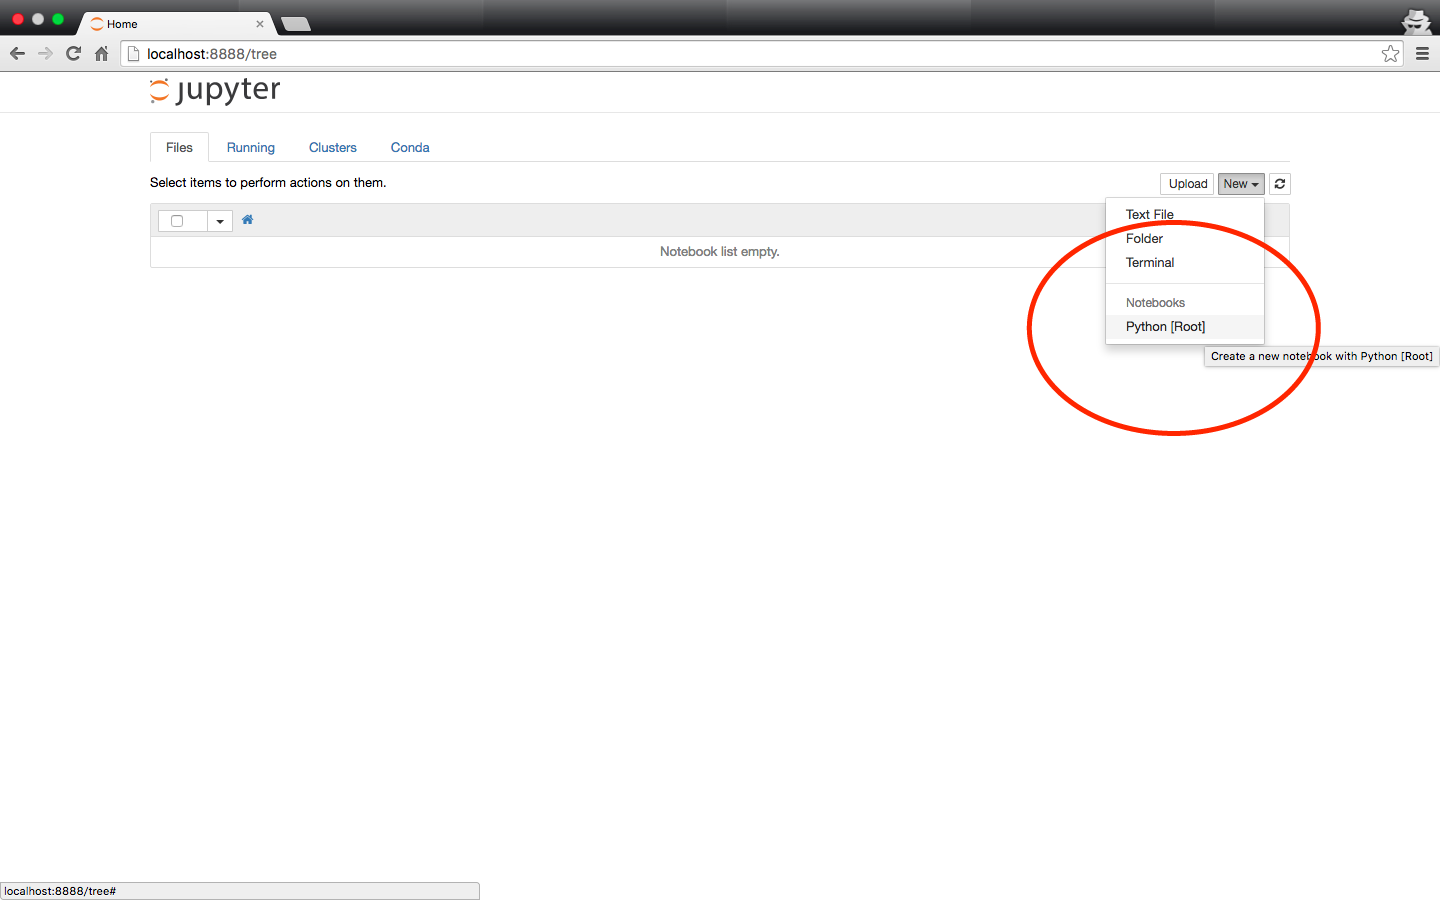
\includegraphics[scale=.25]{graphics/jupyter_10.png}}
\caption{\label{fig: ノートブックの新規作成}%
ノートブックの新規作成.
}
\end{figure}


\subsubsection{既存ノートブックの読み込み}
開きたいノートブック(拡張子ipynbのファイル)
をNotebook Dashboardから選択する.


\subsubsection{Pythonコードの入力}
Notebook Editorにおいて以下のように操作する.
\begin{enumerate}
\item
コードを入力したいセルを選択する.
\item
ツールバーのプルダウンメニューにおいて
セルタイプ「Code」が選択されていることを確認する.
セルタイプが「Code」以外になっている場合は,
プルダウンメニューからセルタイプ「Code」を選択するか,
コマンドモードに切り替えてキーボードショートカット[y]を使用する.
\item
編集モードに切り替え,セルにコードを入力する
(図\ref{fig: Pythonコードの入力}).

\begin{figure}[htbp]
\centering
\setlength{\fboxsep}{0pt}
\fcolorbox{gray}{gray}{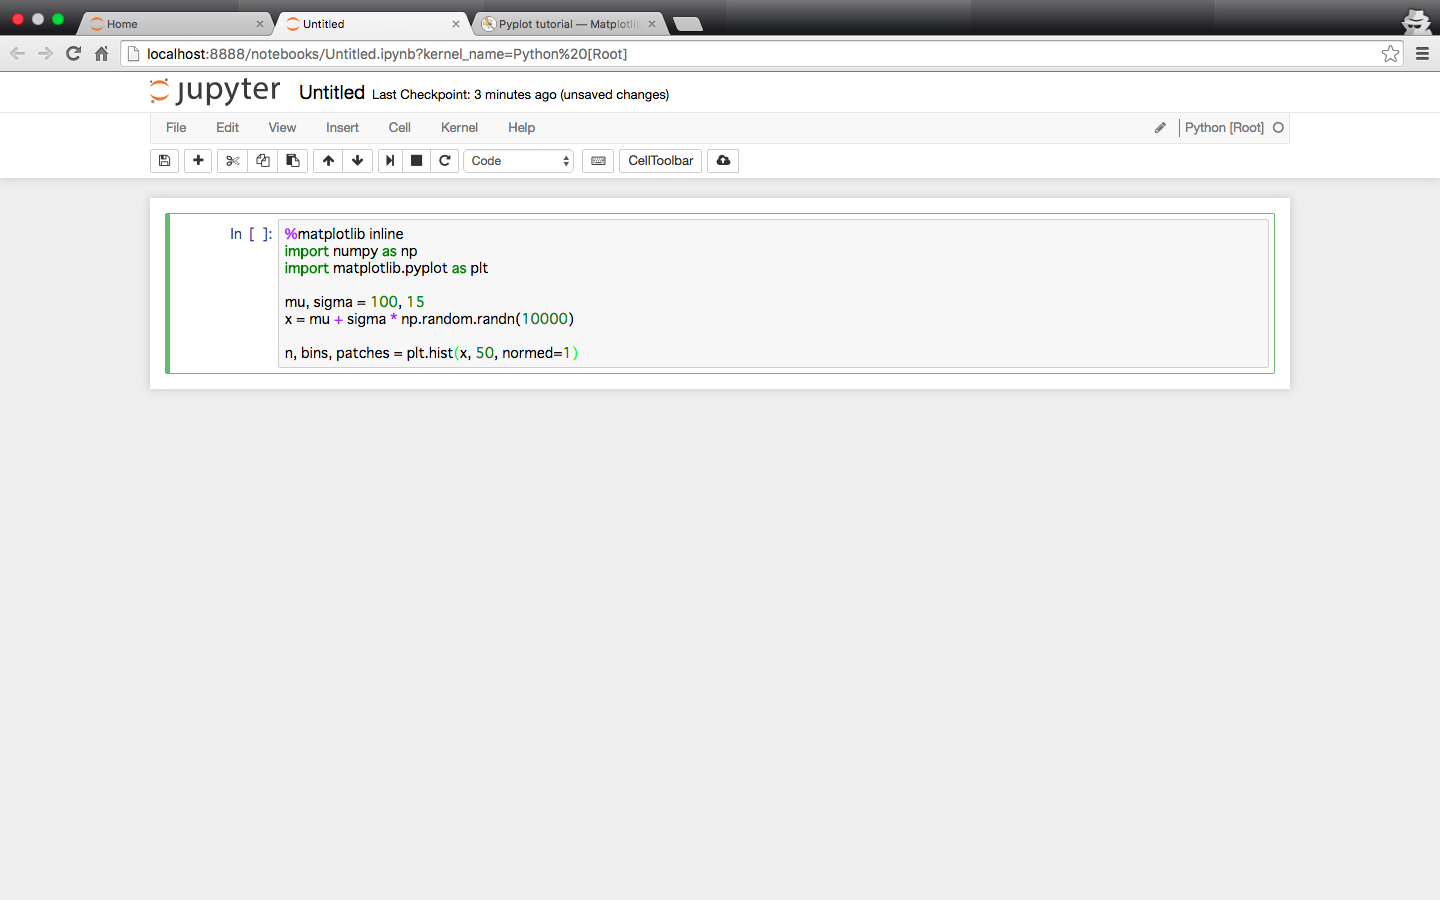
\includegraphics[scale=.25]{graphics/jupyter_06.png}}
\caption{\label{fig: Pythonコードの入力}%
Pythonコードの入力.
}
\end{figure}
\end{enumerate}


\subsubsection{Pythonコードの実行}
Notebook Editorにおいて以下のように操作する.
\begin{enumerate}
\item
実行したいコードが入力されたセルを選択する.
\item
ツールバーの[\,\faStepForward\,]ボタンを押すか,
キーボードショートカット[Shift]+[Enter]
(コマンドモード/編集モードのいずれでも使用可)
を使用する.
実行中のセルはセル番号が\verb|In [*]|と表示される.
\end{enumerate}


\subsubsection{ノートブック名の変更}
Notebook Editorの上部,Jupyterロゴの横に表示されている
ノートブック名をクリックし,
新しいノートブック名を入力する
(図\ref{fig: ノートブック名の変更}).

\begin{figure}[htbp]
\centering
\setlength{\fboxsep}{0pt}
\fcolorbox{gray}{gray}{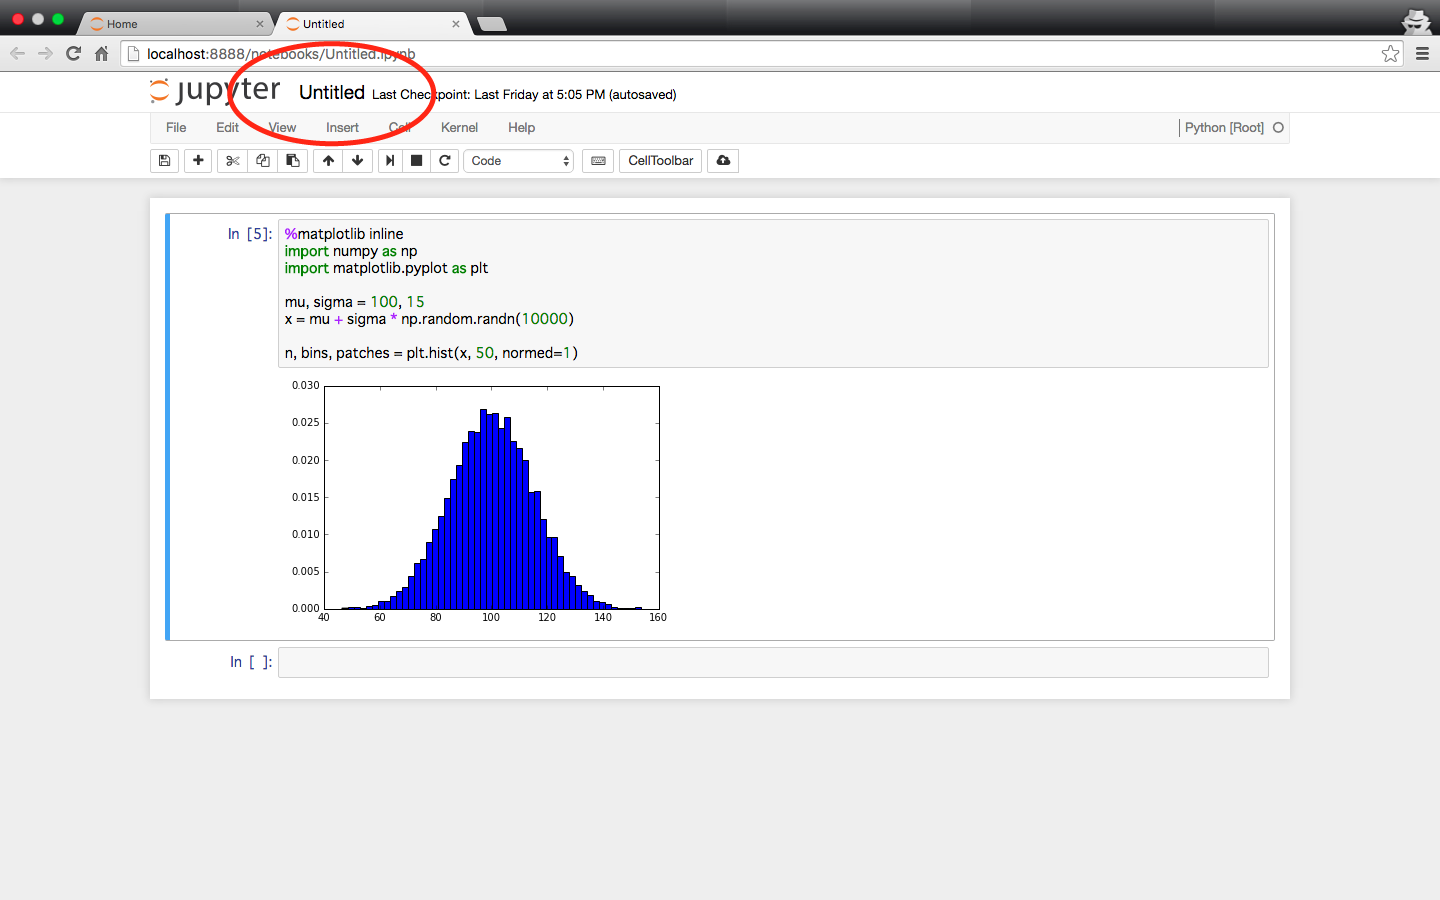
\includegraphics[scale=.25]{graphics/jupyter_12.png}}
\caption{\label{fig: ノートブック名の変更}%
ノートブック名の変更.
}
\end{figure}


\subsubsection{ノートブックの上書き保存}
Notebook Editorにおいて,
ツールバーの[\,\faFloppyO\,]ボタンを押すか,
コマンドモードに切り替えてキーボードショートカット[s]を使用する.


\subsubsection{ノートブックの別名保存}
Notebook Editorの[File]メニューから[Make a Copy...]を選択する.


\subsubsection{Jupyter Notebookの終了}
\begin{enumerate}
\item
Notebook Editorの[File]メニューから[Close and Halt]を選択することで,
Notebook Editorを閉じると同時に計算エンジンを停止させる\footnote{%
計算エンジンを停止させずにNotebook Editorを閉じてしまった場合は,
Notebook Dashboardの[Running]タブを開き,
当該ノートブックの[Shutdown]ボタンを押して停止させる.
}.
\item
Notebook Dashboardを閉じる.
(ブラウザを閉じればよい.)
\item
シェル(コマンドプロンプトもしくはターミナル)
上に残ったサーバジョブを[Ctrl]+[c]キーで停止させる.
\end{enumerate}


\begin{thebibliography}{9}
\bibitem{rossant2015ipython}
Cyrille Rossant(著), 菊池彰(訳)『IPythonデータサイエンスクックブック: 対話型コンピューティングと可視化のためのレシピ集』(オライリージャパン).
\end{thebibliography}


% Pythonプログラミングのヒント
\section{Pythonプログラミングのヒント}\label{sec: Pythonプログラミングのヒント}


\subsection{MATLABデータの読み込み}
	 PythonではMatlabのデータも扱うことができる.ここではその方法を記す.例えば,次のような構造体sが保存されたバージョンが7以前のMatlabファイル`test.mat'を考える.
	\begin{itemize}
		\item s.label =[`node1',`node2'] : 2$\times$5 char
		\item s.samplingrate = 0.05
		\item s.DATA : 2$\times$5$\times$2 double
			\begin{eqnarray*}
				{\rm s.DATA}(:,:,1)= 
					\begin{array}{ccccc}
						1 & 2 & 3 & 4 & 5\\
						6 & 7 & 8 & 9 & 10\\
					\end{array}, 
				{\rm s.DATA}(:,:,2)=
					\begin{array}{ccccc}
						11 & 12 & 13 & 14 & 15\\		
					16 & 17 & 18 & 19 & 20\\
					\end{array}
			\end{eqnarray*}
		\item s.average = [3,8;13,18] : 2$\times$2 double
	\end{itemize}
	このようなMatlabファイルを読み込むにはscipy.ioにあるloadmatを使えばよい.
\begin{lstlisting}[style=python]
d=scipy.io.loadmat(`$ファイル名')
\end{lstlisting}
	と読み込んだ変数dに対して,d[`\$変数名'][0,0][`\$フィールド名']とすれば構造体に含まれているフィールドの値を取得することができる.実際にtest.matを用意した上でコード\ref{code: loadmatのサンプル}を実行すると上記で記した構造体sが読み込まれていることを確認できる.
	\lstinputlisting[%
	style=python,%
	label={code: loadmatのサンプル},%
	caption={loadmatを用いて構造体sを読み込むコード.各フィールドの値を表示する.}]{code/loadmat.py}
	 他方でMatlabファイルのバージョンが7.3であれば,loadmatでファイルを読み込むことができない.この場合はパッケージh5pyを用いることになる.このh5pyはデフォルトではpythonには導入されていないのでh5pyをインストールする.	\begin{lstlisting}[style=cmdline]
> conda install h5py
\end{lstlisting}
	そしてh5pyにあるFileを用いて,
\begin{lstlisting}[style=python]
d=h5py.File(`$ファイル名','r')
\end{lstlisting}
	とすればよい.このようにして読み込んだdに対して,d[`\$変数名/\$フィールド名']のようにすれば構造体に含まれているフィールドの値を取得することができる.ただし,loadmatのときとは異なり,フィールドの値取得後の文字列の形式・次元の向きには注意が必要である.実際にバージョンが7.3であるtest.matを用意した上でコード\ref{code: h5pyのサンプル}を実行すると上記で記した構造体sが読み込まれていることを確認できる.これらのMatlabファイルの読み込みに関する詳細としてはリンク集にあるScipyのドキュメントおよびh5pyのドキュメントを参考されたい.
	\lstinputlisting[%
	style=python,%
	label={code: h5pyのサンプル},%
	caption={h5pyを用いて構造体sを読み込むコード.各フィールドの値を表示する.}]{code/h5py.py}
\subsection{図のファイル出力}
	図のファイル出力はmatplotlib.pyplotにあるsavefigを使えばよい.使い方としては,コード1におけるplt.plot()の部分を
\begin{lstlisting}[style=python]
plt.savefig('$ファイル名')
\end{lstlisting}
	とすればよい.出力画像のフォーマットとしては
	\begin{center}
		eps, pdf, pgf, png, ps, raw, rgba, svg, svgz
	\end{center}
	などが可能である.
\subsection{リンク集}
	\begin{itemize}
		\item PythonJapan(\url{http://www.python.jp/}):Pythonの日本語ドキュメント
		\item SciPy.org(\url{https://docs.scipy.org/doc/}):NumpyとScipyのドキュメント
		\item Matplotlib(\url{http://matplotlib.org/}):Matplotlibのドキュメント
		\item HDF5 for Python(\url{http://docs.h5py.org/}):h5pyのドキュメント
	\end{itemize}





\end{document}
